% ============================================================
%  CONTROL LOOP  –  versione finale pulita
% ============================================================
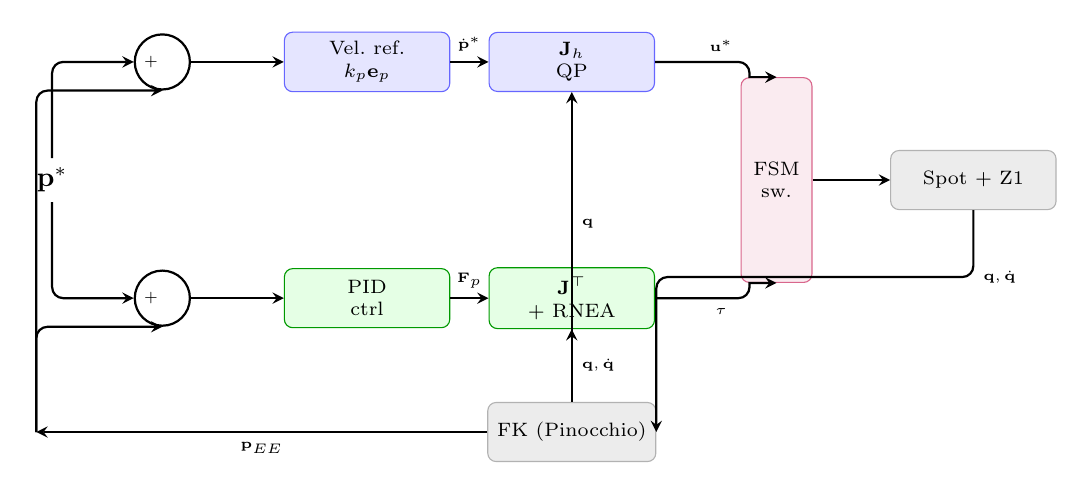
\begin{tikzpicture}[
    >=stealth,
    arr/.style  = {->, thick, rounded corners=4pt},
    box/.style  = {rectangle, draw, rounded corners=3pt,
                   minimum width=2.1cm, minimum height=0.75cm,
                   font=\scriptsize, align=center, fill=white},
    wbc/.style  = {box, fill=blue!10,  draw=blue!60},
    imp/.style  = {box, fill=green!10, draw=green!60!black},
    rob/.style  = {box, fill=gray!15,  draw=gray!60},
    sw/.style   = {rectangle, draw=purple!60, fill=purple!8,
                   rounded corners=3pt, font=\scriptsize, align=center,
                   minimum width=0.9cm, minimum height=2.6cm},
    sum/.style  = {circle, draw, thick, minimum size=0.7cm,  % aumentato size
                   inner sep=0pt, font=\small},
  ]

  % ── Colonne x: -0.2  1.2  3.8  6.4  9.0  11.5 ──────────────
  % ── Righe  y: top=1.5  bot=-1.5  fb=-3.2 ────────────────────

  % INPUT (stesso)
  \node (ref) at (-0.2, 0) {$\mathbf{p}^*$};

  % SUM NODES (size +0.1cm per più spazio interno)
  \node[sum] (e1) at (1.2,  1.5) {};
  \node[sum] (e2) at (1.2, -1.5) {};

  % WBC / IMP / SW / ROBOT / FK  (stessi)
  \node[wbc] (vdes) at (3.8,  1.5) {Vel.\ ref.\\$k_p \mathbf{e}_p$};
  \node[wbc] (jh)   at (6.4,  1.5) {$\mathbf{J}_h$\\QP};
  \node[imp] (pid)  at (3.8, -1.5) {PID\\ctrl};
  \node[imp] (jtc)  at (6.4, -1.5) {$\mathbf{J}^\top$\\+ RNEA};
  \node[sw]  (sw)   at (9.0,  0)   {FSM\\sw.};
  \node[rob] (robot) at (11.5, 0)  {Spot + Z1};
  \node[rob] (fk) at (6.4, -3.2) {FK (Pinocchio)};

  % ── ref → sums ───────────────────────────────────────────────
  \draw[arr] (ref.north) |- (e1.west);
  \draw[arr] (ref.south) |- (e2.west);

  % ── WBC path ─────────────────────────────────────────────────
  \draw[arr] (e1) -- (vdes);
  \draw[arr] (vdes) -- node[above, font=\tiny]{$\dot{\mathbf{p}}^*$} (jh);

  % ── jh → sw:  orizzontale lunga + sharp corner + verticale corta ─
  \draw[arr] (jh.east) 
             -- ++(1.2,0)     % orizzontale ampia, pulita
             node[above, pos=0.7, font=\tiny]{$\mathbf{u}^*$}
             [sharp corners] |- (sw.north);  % sharp solo qui!

  % ── Impedance path ───────────────────────────────────────────
  \draw[arr] (e2) -- (pid);
  \draw[arr] (pid) -- node[above, font=\tiny]{$\mathbf{F}_p$} (jtc);

  % ── jtc → sw:  simmetrico a sopra ────────────────────────────
  \draw[arr] (jtc.east) 
             -- ++(1.2,0)     % orizzontale ampia
             node[below, pos=0.7, font=\tiny]{$\boldsymbol{\tau}$}
             [sharp corners] |- (sw.south);

  % ── switch → robot / robot → FK  (stessi) ───────────────────
  \draw[arr] (sw.east) -- (robot.west);
  \draw[arr] (robot.south) -- ++(0,-0.85)
             node[right, font=\tiny]{$\mathbf{q},\dot{\mathbf{q}}$}
             -| (fk.east);

  % ── FK → Jacobians  (stessi) ─────────────────────────────────
  \draw[arr] (fk.north) -- (jtc.south)
             node[midway, right, font=\tiny]{$\mathbf{q},\dot{\mathbf{q}}$};
  \draw[arr] (fk.north) -- ++(0,0.6) -| (jh.south)
             node[near end, right, font=\tiny]{$\mathbf{q}$};

  % ── FK → sums  (feedback unificato) ──────────────────────────
  \coordinate (fbL) at (-0.4, -3.2);
  \draw[arr] (fk.west) -- (fbL)
             node[midway, below, font=\tiny]{$\mathbf{p}_{EE}$};
  \draw[arr] (fbL) |- (e1.south);
  \draw[arr] (fbL) |- (e2.south);

  % ── + VISIBILI  sui centri, con left=-2pt per entrare nel cerchio ─
  \node[left=-2pt, font=\tiny] at (e1.center) {$+$};
  \node[left=-2pt, font=\tiny] at (e2.center) {$+$};

\end{tikzpicture}
